%!TEX root = ../Thesis.tex

\section{GPS Satellite Signals}
The are two frequencies that GPS uses; L1 frequency at 1575.42 MHz and L2 at 1227.60 MHz \cite{signal spec}. There are two sets of signals that are sent from every satellite, the pseudorandom binary sequence (PRN code) and the navigation message.

\subsection{PRN}
Coarse Acquisition Code, or C/A code, is transmitted on the L1 frequency as a 1.023 MHz signal of 1023 bits. Civilians have access to the C/A code and is what is used in receivers. There is another code modulated onto the L1 and L2 frequencies called the P (Precise) code as a 10.23 MHz signal \cite{CA_oxts}. As it is 10 times faster it is more accurate, and is restricted to military use. Both of these codes are modulated as pseudo random number (PRN) codes and repeat constantly, which have the property of the appearance of random noise but are very precisely defined. It is because it is precisely defined, the GPS receiver can recreate the PRN code at the same time the satellite does. By comparing the incoming signal and the self-generated code the time delay is measured, see Figure \ref{fig:PRNtime}. As the C/A code repeats every millisecond, only a time range of 1 ms needs to be searched \cite{trimble_PRN}.


\cite{mit_signals}

\begin{figure}
\centering
\caption{Pseudorange measurement from the time delay of the PRN code \cite{whatwhenhow}}
\label{fig:PRNtime}
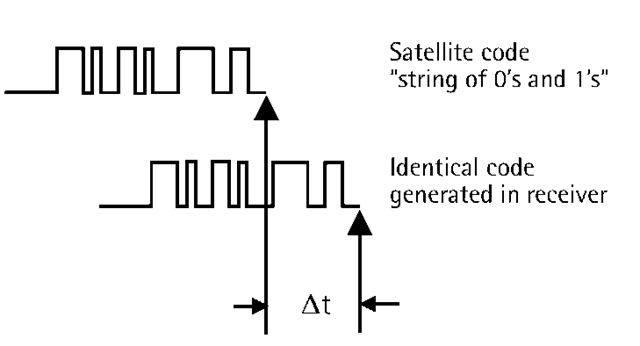
\includegraphics[width=0.7\linewidth]{ChapterLiteratureReview/PRNtime.png}
\end{figure}



\subsection{Navigation Message}
The navigation message is a low frequency signal added to the L1 code at a rate of 50 bps. It has three components \cite{signalspec};
\begin{enumerate}
\item GPS date and time with satellite status at the time the signal was sent
\item Ephemeris data: valid for up to 4 hours
\item Almanac data: valid for 180 days
\end{enumerate}
The almanac data 


\begin{figure}
\centering
\caption{Navigation Message Content and Format Overview \cite{signalspec}}
\label{fig:NavMessage}
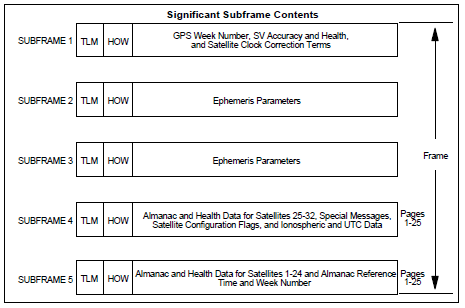
\includegraphics[width=0.7\linewidth]{ChapterLiteratureReview/NavMessage}
\end{figure}



\subsection{Raw Data}
There is a lot of data contained in the total signal, but the following are what is important to this thesis:
\begin{itemize}
	\item \textbf{Time received}: The time in the receivers frame that the sample reading was taken.
	\item \textbf{Pseudorange}: The range calculated by the receiver to the satellite. Depending upon the type of receiver, this measurement may have already been adjusted for some errors that were encoded in the navigation message.
	\item \textbf{Carrier Phase}: The phase of the carrier signal at the receivers point in time.
	\item \textbf{Doppler Shift}: The instantaneous Doppler frequency of the signal. 
	\item \textbf{Satellite Epoch}: The time the signal was sent from the satellite, decoded from the navigation message.
	\item \textbf{Ephemeris Data}: The orbital parameters necessary to calculate the position of the satellite.
\end{itemize}


%The first row shows a C/A code with 1,023 chips; the total length is 1 ms. The second row shows a navigation data bit that has a data rate of 50 Hz; thus, a data bit is 20 ms long and contains 20 C/A codes. Thirty data bits make a word that is 600 ms long as shown in the third row. Ten words make a subframe that is 6 seconds long as shown in row four. The fifth row shows a page that is 30 seconds long and contains 5 subframes. Twenty-five pages make a complete data set that is 12.5 minutes long as shown in the sixth row. The 25 pages of data can be referred to as a superframe http://read.pudn.com/downloads85/ebook/326017/Fundamentals%20of%20Global%20Positioning%20System%20Receivers/booktext05.pdf (pg77)

% resources about the signals:
% http://geoconnect.com.au/gps-signals-l1-l2-l5/
% http://www.trimble.com/gps_tutorial/dgps-advanced4.aspx
% https://www.e-education.psu.edu/natureofgeoinfo/c5_p14.html
% http://what-when-how.com/gps/gps-details/
% https://www.e-education.psu.edu/geog862/node/1742
% http://indico.ictp.it/event/a09138/session/24/contribution/14/material/0/0.pdf
% http://read.pudn.com/downloads85/ebook/326017/Fundamentals%20of%20Global%20Positioning%20System%20Receivers/booktext05.pdf
% http://www.navipedia.net/index.php/GPS_Navigation_Message